%\documentclass[12pt,oneside]{fithesis2}		% pc version
\documentclass[a4paper, 12pt, twoside]{fithesis2}		% print version

% ===== LOADING PACKAGES =====
% language settings, main documnet language last
\usepackage[english]{babel}
% enabling new fonts support (nicer)
\usepackage{lmodern}
% setting input encoding
\usepackage[utf8]{inputenc}
% setting output encoding
\usepackage[T1]{fontenc}
% fithesis2 requires csquotes
\usepackage{csquotes}
% set page margins
%\usepackage[top=3.0cm, bottom=3.5cm, left=2.4cm, right=2.4cm]{geometry}	% pc version
\usepackage[top=3.0cm, bottom=3.5cm, left=2.9cm, right=1.9cm]{geometry}	% print version
% package to make bullet list nicer
\usepackage{enumitem}
% math symbols and environments
\usepackage{mathtools}
\usepackage{amsmath}
% packages for complex tables
%\usepackage{tabularx}
%\usepackage{multirow}
%\usepackage{dcolumn}
%\usepackage{array}
% package for defining new floating environments
\usepackage{float}
\usepackage[labelfont=]{caption}
%\usepackage{newfloat}

% indentation
% vertical space between paragrahps, no indentation
%\usepackage[parfill]{parskip}  % TODO: nefunguje -> zfunkcnit
% space between paragraphs
\setlength{\parskip}{0.6em plus0.2em minus0.2em} % zkraceni vzdalenosti mezi odstavci

% listings for SPARQL
\usepackage{listings}
\lstset{%
  language=SQL,%
  morekeywords={PREFIX,LIMIT},%
  basicstyle=\small\ttfamily,
  frame=single%
}

% bibliography management
\usepackage[backend=biber, 		% use biber as backend instead of BiBTeX
        %dashed=false                    % when there is an author twice, still write his/her name
	bibstyle=ieee-alphabetic, 	% bibliography style: IEEE with alphabetic citations
	citestyle=alphabetic, 		% citation style
	url=true, 			% display urls in bibliography
	hyperref=auto,			% detect hyperref and create links
	%block=ragged, 			% format bibliography into blocks, ragged on right
]{biblatex}
\addbibresource{thesis.bib}

% setting custom colors for links
\usepackage{xcolor}
\definecolor{dark-red}{rgb}{0.6,0.15,0.15}
\definecolor{dark-green}{rgb}{0.15,0.4,0.15}
\definecolor{medium-blue}{rgb}{0,0,0.5}
% generating hyperlinks in document
\usepackage{url}
\usepackage[plainpages=false, 	    % get the page numbering correctly
            pdfpagelabels, 	    % write arabic labels to all pages
            unicode,	 	    % allow unicode characters in links
            colorlinks=true, 	    % use colored links instead of boxed (pc version)
            %hidelinks, 		    % hide links (print version)
            linkcolor={dark-red},
            citecolor={dark-green},
            urlcolor={medium-blue}
			]{hyperref}

% ===== FI THESIS SETTINGS =====

\thesistitle{Automatic Question Generation\\and Adaptive Practice}
\thesissubtitle{Bachelor thesis}
\thesisstudent{Tomáš Effenberger}
\thesiswoman{false}
\thesisfaculty{fi}
\thesisyear{spring 2015}
\thesisadvisor{RNDr.\ Jan Rygl}
\thesislang{en}

% ===== LATEX DOCUMENT SETTINGS =====

% adjusting hyphenation penalties
%\tolerance=10000
%\hyphenpenalty=500

% hyphenations settings
\hyphenation{DBpedia}

% renew command for shorter and nicer underscore
\renewcommand{\_}{\leavevmode \kern0.0em\vbox{\hrule width0.4em}}


% ===== COMMANDS =====

%--------------------------------------------------------------------
% define square symbol
%--------------------------------------------------------------------
\newcommand{\squarebullet}{\textcolor{black}{\raisebox{0.15em}{\rule{4pt}{4pt}}}}

%--------------------------------------------------------------------
% define new itemize environment with squares and smaller spaces
%--------------------------------------------------------------------
\newenvironment{myItemize}{
  \begin{itemize}[leftmargin=2em,rightmargin=1em,itemsep=\parskip ,parsep=0em,topsep=0em,partopsep=0em]
  \renewcommand{\labelitemi}{\squarebullet}
  \renewcommand{\labelitemii}{$\diamond$}
}{
  \end{itemize}
}

%--------------------------------------------------------------------
% exercise environment
%--------------------------------------------------------------------
\newcounter{choice}
\renewcommand\thechoice{\Alph{choice}}
\newcommand\choicelabel{\thechoice.}

\newenvironment{choices}%
  {\vspace{0.2em}\list{\choicelabel}%
     {\usecounter{choice}\def\makelabel##1{\hss\llap{##1}}%
       \settowidth{\leftmargin}{W.\hskip\labelsep\hskip 0.01em}%
       \def\choice{%
         \item
       } % choice
       \labelwidth\leftmargin\advance\labelwidth-\labelsep
       \topsep=0pt
       \partopsep=0pt
     }%
  }%
  {\vspace{-0.7em}\endlist}

%\setlength{\abovecaptionskip}{25pt plus 3pt minus 2pt}
\floatstyle{boxed}
\newfloat{exercise}{thp}{exrcs}[chapter]
\floatname{exercise}{Exercise}

\newenvironment{question}
{
  \begin{center}
  \begin{tabular}{p{0.9\textwidth}}
  \vskip 0.05em
}
{
  \\
  \end{tabular}
  \end{center}
}

% gap in the sentence (bottom line)
\newcommand{\sentenceGap}{\rule{1.5cm}{0.4pt}~}

%--------------------------------------------------------------------

% ===== CHEAT SHEET =====

% == full width image

%\begin{figure}[b!]
%\centering
%\includegraphics[width=\textwidth]{images/bla.bla}
%\caption{bla bla bla}
%\label{fig:bla-bla}
%\end{figure}


% == myItemize

%\begin{myItemize}
%\item \textbf{Bla}\\
%  bla
%\item \textbf{Bla}\\
%  bla
%\item \textbf{Bla}\\
%  bla
%\end{myItemize}


% ===== BEGIN DOCUMENT =====
\begin{document}

\FrontMatter
\ThesisTitlePage

\begin{ThesisDeclaration}
\DeclarationText
\AdvisorName
\end{ThesisDeclaration}

\begin{ThesisThanks}

  TODO (Sir, Papi, ALG, NLP)
%I'd like to thank Petr for his guidance, enthusiasm and inspiring discussions.
%I also owe much to my mom and brother for their continuous support. Thank you.

%\noindent
%Further thanks goes to all my friends who had to put up with my enthusiasm
%and numerous research details they may have never asked for $\ddot\smile$.

%\noindent
%Last but not least, I'd like to acknowledge the Laboratory of Security and Applied Cryptography and
%the National Grid Infrastructure MetaCentrum for providing access to their computing and storage facilities.
\end{ThesisThanks}

\begin{ThesisAbstract}
When studying, it is more efficient not just to read about the topic, but also to practice the knowledge, e.g. by answering some multiple choice questions. Today, there is a huge amount of information to study (consider Wikipedia) and it is not possible to create a set of question for all topics manually. However, we can generate questions automatically, using techniques of artificial intelligence and natural language processing. This thesis explores the state-of-the-art approaches to question generation and describes their advantages and disadvantages. The thesis also suggests a design of the general framework for practicing knowledge from articles. This framework is implemented and publicly accessible through a web interface.
\end{ThesisAbstract}

\begin{ThesisKeyWords}
% TODO: profiltrovat na ty opravdu relevantni
knowledge representation, question generation, adaptive practice, learning,
multiple choice questions
%artificial intelligence, natural language processing,
\end{ThesisKeyWords}

\MainMatter
\tableofcontents

% ===========================  CHAPTER ===========================
\chapter{Introduction}
\label{chap:intro}

TODO: intro, goal of the thesis (dodelat podle oficialniho zadani / abstraktu)

Mere repeated reading of the text which one is traying to learn is unefficient method of learning, while answering to related questions leads to [better long-term knowledge / dlouhodobemu zapamatovani] \parencite{edu-improve}.

TODO: 2 ruzne cile: procvicovani (uceni) tematu vs. testovani; i pri procvicovani tematu muzu chtit i to testovani (abych vedel, jak na tom jsem) (budu se venovat obema (?) a v implementovanem systemu to bude nekde na pomezi)

TODO: neco o tom, ze vytvaret testy manualne je time-consuming, takze by bylo fajn to autmatizovat

In spite of active and [dlouhodoby nebo tak neco] research of question generation
(e.g. \parencite{questions-wolfe, questions-eval}) [mozna pridat dalsi, pripadne rozepsat - priklad early research a recent research],
there is still no publicly available web application to solve this task.
And I am sure that such application would be really useful. Typical example is to make self-studying more efficient by answering a few generated questions after reading an article to verify and consolidate the new knowledge.
[overit aktualnost a jasne urcit moment o kterem mluvim (neexistuje tady a ted)]

That is why I have implemented \textit{Smartoo, Smart Artificially Intelligent Tutor}, modular and extensible framework for question generation and adaptive practice
of knowledge from \emph{Wikipedia}%
\footnote{\url{http://en.wikipedia.org/}}
articles.
The Smartoo Framework is licensed under the GNU General Public License, version 2 [citovat?, licenci rozmyslet].
The source code is available from project's page on \textit{GitHub}.%
\footnote{\url{http://github.com/effa/smartoo}}
I have used the framework to create a simple [instance/demo/prototype?] of the web application for practicing knowledge from Wikipedia articles.%
\footnote{\url{http://smartoo.thran.cz}}

The whole practicing process consists of four steps.
First step is to extract facts from the given article.
Besides the knowledge extraction itself, knowledge representation is an important issue as well.
Extraction and representation of the knowledge is the topic of \autoref{chap:knowledge}.

In \autoref{chap:exercises}, excercises generation is discussed.
Usually, exercises will be just multiple choice questions, but other exercises types are possible as well.
In this step major concerns are: selection of a fact (or set of facts) from which the exercise will be generated, transformation from the fact (or facts) to the exercise and in case of multiple choice questions selection of good \textit{distractors} (incorrect choices).

TODO: upravit podle aktualniho rozdeleni na kapitoly: Although we could stop here and submit all generated questions to the user, it has been proven to be useful to make two more steps.
In \autoref{chap:exercises-grading}, I talk about exercises grading.
We can be interested in various parameters, such as difficulty, relevance to the article or probability that the question is gramatically [?].

Having the exercises graded, we can filter them and only present these with reasonable difficulty, relevance and correctness probability.
But again, we can introduce one more step to make learning more efficient -- adaptive practice.
According to the user performance, we can choose easier or more difficult questions. I talk about some common strategies for this task in \autoref{chap:practice}.

In \autoref{chap:smartoo}, I describe the Smartoo Framework in detail
and we will see how these four steps are transparently glued and how a component for each step should look like.
I also mention how each of the four components is implemented in the online prototype system.

Smartoo is designed to collect both implicit and explicit feedback from users.
I analyze feedback from about one month testing period in \autoref{chap:evaluation}.

Finally, in the \autoref{chap:future}, I present planned future development of Smartoo application.


%The thesis text was typeset in \LaTeX{} using the \textit{fithesis2} package created by Stanislav Filipčík \parencite{fithesis}.

%TODO: (?) The text of the thesis is licensed under a Creative Commons Attribution 3.0 Unported License.


% ===========================  CHAPTER ===========================
\chapter{Knowledge Extraction and Representation}
\label{chap:knowledge}

Knowledge extraction is well-studied aria \parencite{triples-acquisition}.

TODO... rozebrat ruzne pistupy


TODO: zminit omezeni na zachyceni faktu, ne "procedural knowledge" jako je napr. pocitani prikladu a dalsi "higher order cognitive skills"



TODO: jasne dat najevo (diagram), ze tato faze neni v zasade nutna (napr. do uvodu)


% ---------------------------  SECTION  ---------------------------
\section{RDF graph}
\label{sec:rdf-graph}

TODO: o co jde (obvykly zpusob reprezentace znalosti)


RDF graph is often used for knowledge representation.

Facts are stored in the form of \textit{RDF} (\textit{Resource Description Framework}) graph [citovat],
which is a collection of subject -- predicate -- object triples \parencite[][63]{semantic-web}. Simple example of few facts about Alan Turing and Alonzo Church:


\begin{verbatim}
Alan Turing - type - person
Alan Turing - birthdate - 23 June 1912
Alan Turing - nationality - British
Alan Turing - doctoral advisor - Alonzo Church
\end{verbatim}

\begin{verbatim}
Alonzo Church - type - person
Alonzo Church - nationality - American
Alonzo Church - birthdate - 14 June 1903
\end{verbatim}

The collection of RDF triples can be thought of as a graph,
where vertices correspond to subjects and objects
and edges represent relations between them.

\begin{figure}[h]
  \centering
  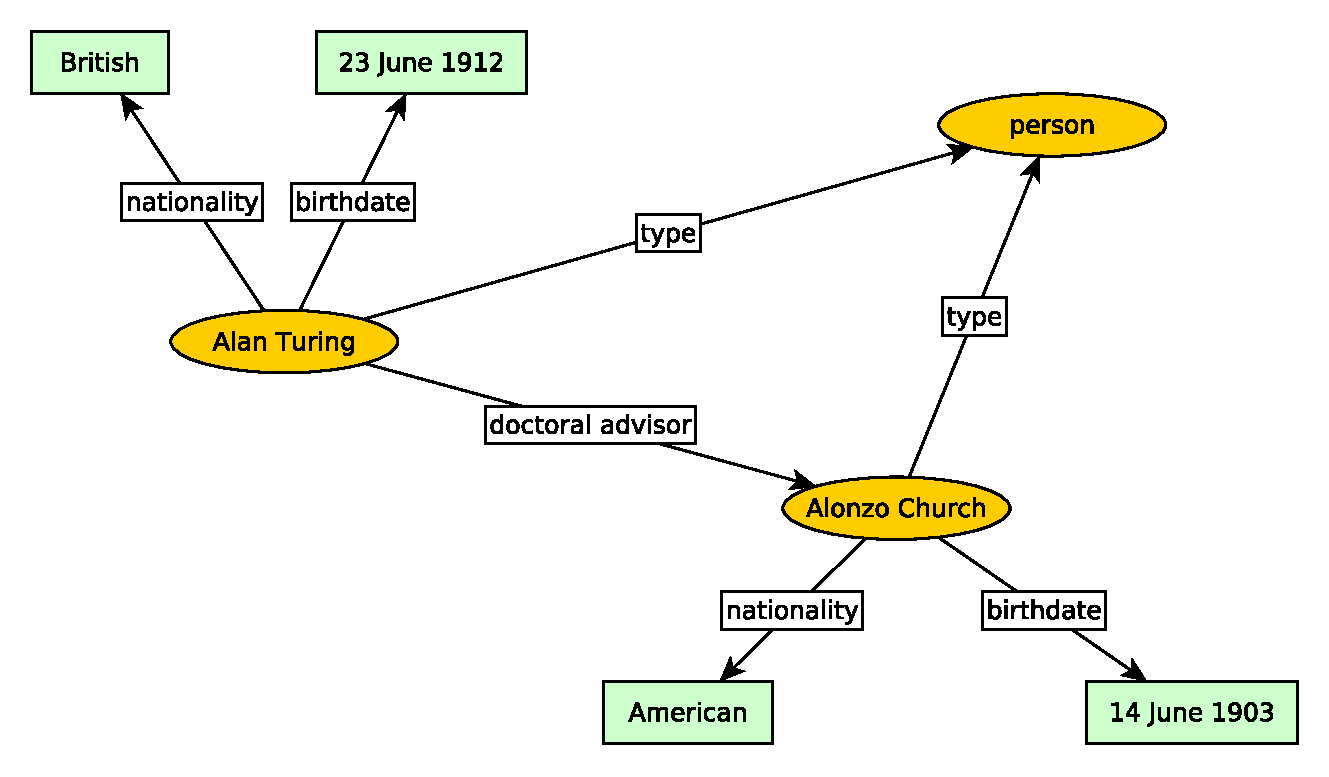
\includegraphics[width=0.9\textwidth]{images/rdf-graph.pdf}
  \caption{Simple RDF graph}
  \label{fig:simple-rdf-graph}
\end{figure}

To avoid possible ambiguity (e.g. between two people who have both name "Alan Turing")
we will use unique URIs%
\footnote{\emph{Uniform Resource Identifier}, TODO: odkaz/vysvetleni}
to represent terms (subjects and objects) and properties (predicates).
URI is composed from a prefix and a name.

\begin{tabular}{ l  l }
  %\hline
  URI & \texttt{http://dbpedia.org/resource/Alan\_Turing}\\
  \hline
  prefix & \texttt{http://dbpedia.org/resource/}\\
  name & \texttt{Alan\_Turing}\\
  %\hline
\end{tabular}

\noindent
Objects can be either URIs or literals, such as number, string or date. (Maybe TODO: priklady)
Simple example with prefixes (part of the graph above):

\begin{verbatim}
<http://dbpedia.org/resource/Alan_Turing>
    <http://www.w3.org/1999/02/22-rdf-syntax-ns#type>
    <http://xmlns.com/foaf/0.1/Person> .
<http://dbpedia.org/resource/Alan_Turing>
    <http://dbpedia.org/ontology/birthDate>
    1912-06-23+02:00
<http://dbpedia.org/resource/Alan_Turing>
   <http://dbpedia.org/property/nationality>
   "British"@en
\end{verbatim}

Or, with the use of seperated definition of URI prefixes (so called \emph{Turtle syntax}):

\begin{verbatim}
@prefix rsrc: <http://dbpedia.org/resource/>
@prefix rdf: <http://www.w3.org/1999/02/22-rdf-syntax-ns#>
@prefix dbpedia-owl: <http://dbpedia.org/ontology/>
@prefix dbprop: <http://dbpedia.org/property/>
@prefix foaf: <http://xmlns.com/foaf/0.1/>

rsrc:Alan_Turing
  rdf:type foaf:person ;
  dbpedia-owl:birthDate 1912-06-23+02:00 ;
  dbprop:nationality "British"@en .
\end{verbatim}

% ---------------------------  SECTION  ---------------------------
\section{SPARQL}
\label{sec:sparql}

\textit{SPARQL}%
\footnote{The name of this query language is a recursive acronym of \textit{SPARQL Protocol and RDF Query Language}.}
is query language for convenient querying of RDF graphs. \parencite[][84]{semantic-web}.

% TODO: seznam ala Martin Ukrop
%SPARQL query resembles SQL query.
The main parts of the query are
\begin{description}
  \item[PREFIX] -- definition of prefixes and assosiated shortcuts
  \item[FROM] -- dataset (RDF graph) on which to run the query
  \item[SELECT] -- which information to return
  \item[WHERE] -- condition on returned data
  \item[ORDER BY] -- ordering of results
\end{description}

As an example, the following SPARQL query would return the birthdate and birthplace of Alan Turing:

\begin{lstlisting}
PREFIX rsrc: <http://dbpedia.org/resource/>
PREFIX owl: <http://dbpedia.org/ontology/>
SELECT ?date ?place
WHERE {
  rsrc:Alan_Turing owl:birthDate ?date ;
                   owl:birthPlace ?place .
}
\end{lstlisting}

% ---------------------------  SECTION  ---------------------------
\section{Ontology}
\label{sec:ontology}

TODO: ontologie - co to je, k cemu to je

TODO: asi nasledovane rozdeleni: obecne info o ontologiich (a jak je generovat) v knowledge kapitole; v kaptiole exercises pak generovani otazek z ontologii

O co jde: ontologií se rozumí popis vlastností, tříd a jejich hierarchie
(mezi tridou a podtridou je "is-a" relationship)

TODO: ukazka ontologie OWL pouzite v DBpedii (Thing, Agent, Person, ...) - to je spis hierarchie trid...

- v dalsi kapitole (odkaz) bude rozebrano, jak generovat otazky s vyuzitim ontologii


% ---------------------------  SECTION  ---------------------------
\section{Terms extraction}
\label{sec:terms-extraction}

TODO: co chapeme termy (named entities), priklady

Pristupy k Terms extraction: napred se text prozene nejakym parserem, ktery identifikuje nouns and noun phrases, spocita se jejich frekvence a ty ktere presahnou nejakou mez, tak se povazuji za pojmy. Tohle teda jako pojmy muze zvolit i obecna casto pouzivana podstatna jmena, ale tohle se pri vyhodnoceni neukazalo jako zasadni problem (naopak varianty jako TF-IDF zahazovali i nemalo pojmu, pokud se tyto casto pouzivaji -- coz bylo u nich docela caste, vzhledem k tomu, ze to testovali na nejakych lingvistickych textech)
\cite{question-gen-mitkov}

Dalsi pristupy (pouzite napr. v \textit{The Mentor} \cite{mentor}): all named entites are find in the text
(using several techniques -- regular expression, gazetteers [odkaz na vysvetleni jinam do textu] and a machine learning-base recognizer as well) (TODO: rozebrat, ukazat priklady)

TODO: dalsi mozne pristupy

% ---------------------------  SECTION  ---------------------------
\section{Relations extraction}
\label{sec:relations-extraction}

TODO... (viz knizka a dalsi clanky)

% ---------------------------  SECTION  ---------------------------
\section{Knowledge Bases}
\label{sec:knowledge-bases}

There are several huge publicly available knowledge bases,
which try to capture as many facts about the world as possible.
Examples of popular knowledge bases are
\textit{DBpedia}\footnote{\url{http://dbpedia.org/}}
and \textit{Freebase}.\footnote{\url{https://www.freebase.com/}}
Knowledge bases are used form many task in natural lanuage processing,
such as named entity recognition (TODO: coz by se melo rozebirat v predhozi kapitole ?!),
desambiguation,
semantic search (Maybe TODO: co to znamena, citovat Google)
and question answering -- several knowledge bases (including DBpedia) were used in \emph{DeepQA project} to create \emph{IBM Watson} computer, which won the \emph{Jeopardy!} quiz game against two human champions in 2011 \cite{watson}. And we can make use of information in these knowledge bases to create better exercises as well. [TODO: upravit posledni vetu, zpresnit, kdy a k cemu budeme bazi znalosti vyuzivat]

DBpedia was built by extracting structured information from Wikipedia,
such as titles, links between articles, external links, information from infoboxes and categories.
Facts are stored in the form of an RDF graph.
Whole knowledge base (TODO: zhruba velikost) can be be downloaded.%
\footnote{\url{http://wiki.dbpedia.org/Downloads}, %
(data available under \emph{Creative Commons Attribution-ShareAlike License}
and \emph{GNU Free Documentation License}}
It also possible to use public \textit{DBpedia SPARQL endpoint}.%
\footnote{\url{http://dbpedia.org/sparql}}

\emph{DBpedia Version 2014}%
\footnote{\url{http://wiki.dbpedia.org/Downloads2014}}
contains approximately 580 million facts (RDF triples) retrieved from the English Wikipedia
\parencite{dbpedia} describing 4.5 million of things.
Ontology of DBpedia includes more than 650 classes and 2700 properties.

TODO: ukazka hierarchie trid, neco na styl nasledujiciho, akorat grafove (obrazkove):

\begin{verbatim}
- Thing
  - Activity
    - Game
    - Sport
  - Agent
    - Deity
    - Family
    - Organization
    - Person
      ...
    ...
\end{verbatim}

% ===========================  CHAPTER ===========================
\chapter{Question Generation}
\label{chap:exercises}

TODO: jasne rict (a mozna diagram), ze jsou 2 zakladni moznosti: bud jsou cviceni generovana primo z textu, nebo je tam ten mezikrok, kdyz se stavi knowledge graph

[Intro, TODO: nejcasteji multiple-choice question, definice, distractory, ukazka]

TODO...

... obecny popis multiple choice questions a souvisejici terminologie (TODO: nejake obecne intro, ze jsou oblibene, maji sve vyhody a nevyhody):

Multiple choice questions consists of a question text (called \textit{stem})
and a few (e.g. four) choices, from which one is the correct answer
and the rest are incoreect alternatives (called \textit{distractors}).

NOTE: asi napred o pristupech ke generovani otazek a distraktory spolecne na konec


% ---------------------------  SECTION  ---------------------------
\section{Syntactic Approach}
\label{sec:questions-syntactically}

TODO: citovat priklady: \textit{AutoQuest} \cite{questions-wolfe}, prehistorie (70. leta), aktualnejsi pak napr. (Mitkov 2006) \cite{question-gen-mitkov}.

TODO popsat: Prvni system jiz v 70. letech -- \textit{AutoQuest} \cite{questions-wolfe}.

TODO: Jeden z moznych postupu (Mitkov, 2006) \cite{question-gen-mitkov}:
extrakce pojmu z textu (pomoci frekvenci), otazky transformaci vet s pojmy (vzory predem dane), vyber distraktoru (snaha o semantickou blizkost odpovedi ... pomoci WordNetu ... viz sekce distractors):
1) terms extraction: identifikace klicovych (domain-specific) pojmu (to budou odpovedi na otazky)
2) stem generation: pretvoreni vety (uvazovany pouze jednoduche vety) v o otazku (step) pomoci jednoduchych transformacnich pravidel
3) distractor selection: z ostatnich pojmu, snaha o co nejvetsi semantickou blizkost (za timto ucelem pouzili WordNet)


Stem generation: z vety se tvori otazka, pokud obsahuje nejaky pojem a navic ma urcitou strukturu, napr.
$$
S V O \text{.} \longrightarrow \text{Which } H V O \text{?}
$$
where $S$, $V$, $O$ stand for \textit{subject}, \textit{verb} and \textit{object} and $H$ is the hypernym of the subject (found using WordNet). (TODO: uvest priklad)

Zajimavost: prvni verze systemu dosahovali komem 5 procent otazek, ktere byly relevantni a bez chyby (tj. ktere se dali pouzit bez uprav).


% ---------------------------  SECTION  ---------------------------
\section{Semantic Approach}
\label{sec:questions-semantically}

Semanticky pristup k tvorbe otazek: \cite{questions-eval}.
Vety jsou nejprve zparsovany a semantic role labeling, napr. kdo je agent, patient etc.
Typy otazek popsane pomoci generickych sablon, ty popisuji vztah mezi vetou a otazkou (s vyuzitim sementickych roli a syntaktickych konstituentu, naprt. \texttt{What |verb| |patient| |location|?} with answer being \texttt{agent} atp., taky. specifikuji semanticou roli, kterou zastava odpoved atp.


% ---------------------------  SECTION  ---------------------------
\section{Lexico-syntactic Patterns}
\label{sec:lexico-syntactic-patterns}


NOTE jeden z moznych pristupu, bootstraping lexikalne syntaktickych vzoru

... The approach of bootstrapping lexico-syntactic patterns was used
in \textit{The Mentor} system \cite{mentor}, created by Technical University of Lisbon.

There are 2 steps.
First, the system learns patterns in sentences which describe a relation between a question and an answer.
After this preparatory offline step, these patterns are used for question generation from texts submitted by users (which is the second step).

The first step uses a few question-answer pairs as seeds.
New sentence-question patterns are boostrapped ....

TODO: popsat blize, co znamena ten bootstrapping

... they are using \textit{QuestionBank} a corpus of 4000 parse-annotated questions \cite{question-bank}.

TODO: svuj vlastni priklad

As an example, consider sentence "Botticelli has painted the Birth of Venus".

General form of pattern is: [TODO, je tam nekde odoved, nejaka pevna cast (*), ktera muze byt pouze jedna, libovolne dlouha a na zbytku jsou urcene vetne cleny (VBD, NP, ...)]

Which of the [uvazovanych] patterns are correct is decided by
Google search of phrase [ktera fraze presne?].

The derived pattern is \texttt{<ANSWER> has VBD NP}.



In the online step, each sentence of given text (after parsing) is matched against boostrapped patterns
and may produce question-answer pair.
Then some filters are applied to discard questions of poor quality. Two main filters are:

\begin{enumerate}
  \item matching question-answer category:
    The category of the question and the category of the answer have to be same (e.g. individual or location). Example: "Who was Abraham Lincoln?" -- "16th president of the United States": both \textit{Abraham Lincoln} and \textit{president} has the semantic category \textit{individual}.
    To find that president is individual, WordNet [citovat] is used (BFS).
  \item Discarding Anaphoric References: e.g. "Where is there?"
\end{enumerate}


NOTE: asi docela uspesne, i kdyz mnoho otazek potreba rucne opravit (nepredpokladalo se online nasazeni)



% ---------------------------  SECTION  ---------------------------
\section{Generating exercises from knowledge graphs}
\label{sec:irt}

TODO: definovani a sjednoceni terminologie: ontologies vs. knowledge graphs

TODO (mozna sekce, mozna vice sekci): o tom, jak z grafu znalosti dostat otazky

- generovani otazek s vyuzitim ontologii:
\cite{question-gen-domain-ontologies} -- popisuje ruzne strategie, jak z hotoveho grafu generovat otazky (coz je v nejjednodussim pripade proste vyber jednoho faktu) a k nim distraktory (i distraktory jen na urovni celych vet, zadani bylo vzdy "Choose the correct sentence"; priklady:
- pro RDF trojici A-B-C vytvor distraktor A-B-D, kde D je typu, ktery je podtridou typu C
- pro RDF trojici A-B-C, pokud je C numericka hodnota, vytvor distraktory jako nasobky (a podnasobky) dane hodnoty;

NOTE: jeste na tom clanku je zajimava tabulku udavajici pocet syntakticky bezchybne vygenerovanych otazek pro ruzne clanky (velky rozptyl... od 5 do 85 procent spravnych otazek ... ale je to relativne stary clanek z pocatku jejich vyzkumu, v tom nasledovnem jiz reportuji, ze 90 procent otazek bylo oznaceno jako "dobrych")

\textit{OntoQue} \cite{ontoque}, a system generating questions from a domain ontology.
Various question types: multiple choice questions, true/false, fill-in the blanks.
True/False: chybne vety jsou ze spravne vety vytvoreny nahrazenim subjektu nebo objektu za term, ktery je semanticky blizko (je ze stejne tridy).


TODO: popsat jak se daji vytvaret zajimavejsi otazky s vyuzitim knowledge graphs (viz Procvicnik, napr. Mohli se potkat?)


% ---------------------------  SECTION  ---------------------------
\section{Distractors}
\label{sec:distractors}

It is important to present a multiple-choice question with competitive \textit{distractors}.
As shown by experiments described in \cite{optimizing-multiple-choice}, multiple choice questions with competitive incorrect alternatives not only help to remember the correct answers to the original questions, but they also improve later performance on the previously nontested questions for which these alternatives may be the correct answers. If the alternatives are not competive, a student can recognize the correct answer without retrieval, just by pattern matching. As an example, consider the following multiple choice question:

\begin{exercise}
\caption{Question with noncompetitive alternatives}%\label{table:somename}
  \begin{question}
  Lincoln was assassinated by \sentenceGap , a Confederate sympathizer.
  \begin{choices}
    \choice Emancipation Proclamation
    \choice John Wilkes Booth
    \choice Illinois
    \choice Department of Agriculture
  \end{choices}
  \end{question}
\end{exercise}

Clearly, the student does not need to remember who assasinated Lincoln to answer this question correctly and they are also not forced to retrieve any knowledge about alternatives.
Of course, this was an extreme example to illustrate the point -- you definitely would not come accross such poor distractors in manually created multiple-choice questions.
Now take a look at the following question:

\begin{exercise}
\caption{Question with competitive alternatives}%\label{table:somename}
  \begin{question}
  Lincoln was assassinated by \sentenceGap , a Confederate sympathizer.
  \begin{choices}
    \choice Thomas N. Conrad
    \choice Robert E. Lee
    \choice John Wilkes Booth
    \choice Ward Hill Lamon
  \end{choices}
  \end{question}
\end{exercise}

This questions is much more likely to force student to retrieve knowledge about John Wilkes Booth as well as about other alternatives.

\cite{optimizing-multiple-choice} also showed that competitive distractors are not confused with correct answers in later questions more often than noncompetitive distractors.

The consequences are clear -- when creating a multiple-choice question, we should try to find plausible alternatives which are as competitive as possible.
A tak se skutecne deje v ruznych aktualnich systemech \cite{question-gen-mitkov, slepe-mapy}
NOTE: u systemu, kde je omezena fixni sada faktu k nauceni (slepe mapy), tak lze brat jako distraktory polozky, ktere se nejvice pletou (citovat slepe mapy).

TODO: konkretni strategie:

1] pokud mam pojmenovane entity textu (odkaz na sekci terms extraction v predchozi kapitole), tak vybrat z nich, a to stejneho typu (napr. osoby, mista atp.) -- citovat pouziti, myslim, ze to bylo v Mentorovi (2 stupnova hierarhcie termu)

2] \cite{question-gen-mitkov}:
pomoci WordNetu: coordinates (= terms sharing at least one hypernym with the correct answer). Pokud se jich ve WordNetu najde mnoho, preferuji se ty, ktere se vyskytuji i v dokumentu. Pokud naopak WordNet nevrati nic, pouziji se jmenne fraze z textu, ktere maji stejnou hlavu (leading noun) jako sparvna odpoved. (Pokud ani toto neexistuje, tak se otazka nevytvori.)


3] distraktory z Knowledge Graphu (ontologii) [presunout povidani ze sekce vyse]




% ===========================  CHAPTER ===========================
%\chapter{Exercises Grading}
%\label{chap:exercises-grading}

%NOTE: mozna neni na samostatnou kapitolu (v tom pripade spojit s predchozi, ale je to tak vice konzistentni

% ===========================  CHAPTER ===========================
\chapter{Adaptive Practice}
\label{chap:practice}

TODO popis stavu: mame vygenerovane otazky (prip. i s ohodnocenim?), ted je chceme studentovi predkladat, v nasem settings: obvykle mame spousty otazek (destiky nebo stovky) ale predlozit jich ma cenu je nekolik (napr. 10 nebo 20, prip. dalsi na zadost uzivatele) ... je tedy dulezite umet vybrat ty nejvice pro studenta relevantni otazky a zaroven vyvazovat prumernou uspesnost (pokud by uzivatel nevedel nikdy spravnou odpoved, tak by ho to deprimovalo)

TODO: trochu jine podminky jsou, pokud jsou otazky (nebo aspon fakta) vytvoreny predem (napr. slepe mapy), ale i tam nas samozrejme zajima adaptabilni procvicovani a mnohe z nasledujiciho se vztahuje k obema pripadum

TODO o co jde: poskytovani tech otazek, ktere jsou pro uzivatele co nejuzitecnejsi ... tj. zamereni na to, co student jeste moc dobre neumi, ale na druhou stranu vyvazovat uspesnost (pokud by uzivatel nevedel na zadnou otazku spravnou odpoved, tak by ho to deprimovalo.

(TODO: mozne rozdeleni na 3 casti: odhad prior knowledge (nejspis na urovni jednoho faktu), odhad aktualni znalosti (ma smysl pri opakovanych otazkach na 1 fakt, napr. slepe mapy, ale nikoliv Smartoo), selection of a suitable question (podle odhadu znalosti a historie odpovedi).)


Takze napred projdu nekolik nejznamejsich zpusobu modelovani skillu studenta a obtiznosti faktu (IRT/Rash, PFA, ELO, PFAE, BKT), pak se zamerim na samotny vyber otazky.


% ---------------------------  SECTION  ---------------------------
\section{Item Response Theory}
\label{sec:irt}


TODO...

NOTE: Mozna zvlast sekce o IRT a Rash Modelu?

Napr. Rash Model, coz je logisticky model, predpoklad konstantni znalosti studenta (neuvazuje uceni). Pro multiple choice questions with $n$ options (tj. pravdepodobnost nahodneho uhadnuti je $\frac{1}{n}$), znalost studenta daneho faktu dana parametrem $s$ a obtiznost tematu dana parametrem $d$, vypada odhad spravne odpovedi nasledovne:

$$
P(correct \mid k, d) = \frac{1}{n} + \left( 1 - \frac{1}{n} \right) \cdot \frac{1}{1 + e^{-(s - d)}}
$$

(Mozne TODO: graf)

TODO: uceni parametru: joint maximum likelihood estimation (odkaz), offline, potreba dost dat a je to pomale a obzvlaste nevhodne pro online aplikace, kde je idealni kontinualni update


% ---------------------------  SECTION  ---------------------------
\section{Performance Factor Analysis}
\label{sec:pfa}

NOTE: Performance Factor Analysis = rozsireni Rash modelu, aby uvazoval meninic se znalost skillu; pravdepodbnost odpovedi je stale dana logaritmickou funkci, ale neni zavisla na konstantnim rozdilu znalosti studenta a obtiznosti faktu, ale na linearni kombinaci obtiznosti a poctu studentovych spravnych a poctu chybnych odpovedi na prislusnou otazku ($m = d + \alpha \cdot correctCount + \beta \cdot incorrectCount$).
Vsimneme si, ze v uvahu nebere poradi spravnych a spatnych odpovedi, pouze jejich obsolutni pocet (tj. neumi rozlisit mezi tim, ze jsem 10 krat odpovedel spatne a pak 10 krat dobre a mezi tim, ze odpovidam jednou dobre a jednou spatne.)

Dalsi problem je, ze nebere v uvahu moznost tipovani (coz je potreba u multiple choice otazek).

% ---------------------------  SECTION  ---------------------------
\section{Elo System}
\label{sec:elo}


TODO: inspirovane hodnocenim sachovych hracu \cite{elo-rating}, mozna i napred trochu popsat, jak to funguje tam a pak teprve ta analogie na nasi situaci

Je to dalsi zpusob, jak rozsirit Rash model o uceni, odhad spravne odpovedi zustava stejny logisticky model (odkaz na ten vzorecek). Skill se updatuje po "zapasu" mezi studentem a otazkou (faktem) nasledovne,
kde $s$ je skill studenta, $R$ je result (1 if the answer was correct, 0 if incorrect).
$$
s \gets s + K \cdot (R - P(R = 1))
$$

NOTE: Lze pouzit (a ve Slepych mapach \cite{slepe-mapy} se pouziva) i pro odhad prior knowledge (a global difficulty faktu)
(Oproti Rash modelu asi nema v tomto ohledu tak dobrou semantiku (viz clanek slepe-mapy), ale zato se lepe pocita, vhodny pro online system; navic experimenty ukazuji, ze se to chova podobne (odkaz opet v clanku ve slepe-mapy).
Pak je ale problem with constant K: kdyz je moc mala, tak je uceni pomale, kdyz je velke, tak nestabilni, je tedy vhodne (a pouziva se v Slepe mapy -- viz \cite{slepe-mapy}, mozna odkaz spis primo na system) pouzit misto konstanty
uncertainty function, e.g. $K = \frac{a}{1 + bn}$, kde $n$ je kolik otazek uz uzivatel zodpovedel (nebo obracene, kolik otazek na dane misto jiz bylo zodpovezeno) a $a$ a $b$ jsou fixne zvolene parametry.

Moznost zkombinovat PFA a Elo (viz \cite{slepe-mapy}, nazyvaji to PFAE, kde E muze znamenat bude Elo nebo Extended), porad stejna logisticka funkce, nyni vzhledem k $K_{sf}$, coz je odhad, ze student $s$ zna fakt $f$. Tato promenna (odhad) se updatuje po kazde otazce studenta $s$ na otazku na fakt $f$ podle vzorce pro Elo (odkaz), akort misto jedne konstanty $K$ se pouzivaji 2 ruzne pri spravne vs. spatne odpovedi.


% ---------------------------  SECTION  ---------------------------
\section{Bayesian Knowledge Tracing}
\label{sec:bayesian-network}

TODO: Baysovska sit (HMM) k popisu konceptu (skill) a jejich nauceni (2 stavy: known (learned) and unknown (unlearned)), 4 parametry modelu: pravdepodobnost, ze je koncept known hned od zacatku, pravdepodobnost nauceni v 1 kroku, pravdepodobnost spravne odpovedi, kdyz koncept neumim (guess) a pravdepodobnost spatne odpovedi, kdyz koncept umim (slip).
Update skillu po odpovedi na otazku: s pouzitim Bayesova pravidla.
Odhad parametru: napr. pomoci Expectation Maximization na existujicich datech.

Predpoklad je diskretni prechod z neumim do umim (coz je obvykle dost zjednodusujici, zapamatovani deklarativnich faktu je postupne).

Priklad systemu pro uceni, ktery vyuziva BKT: \cite{question-gen-adapt-bayes} (trochu rozebrany nize).

TODO: Dalsi clanky viz odkazy v clanku slepe-mapy.


% ---------------------------  SECTION  ---------------------------
\section{Question selection}
\label{sec:question-selection}

NOTE: predchozi sekce (mozna to mely byt jen podsekce, ale to je jedno) se zabyvaji, tim, jak modelovat znalost studenta a obtiznost konceptu/faktu. To je jedna z komponent, kterou pro vyber vhodne otazky potrebujeme.

Kriteria, ktera jsou dulezita pro vyber vhodne otazky:

\begin{myItemize}
  \item relevance -- obecne relevance pro studenta, v nasem kontextu hlavne relevance k danemu tematu, v jinem to muze znamenat vice aktualni relevanci - co zrovna ted potrebuje student procvicit nejvice (least known concept -- napr. \cite{question-gen-adapt-bayes} ... neni potreba uplne resit pokud cekam, ze tam bude uzivatel dost dlouho a casem se dostnane ke vsemu)
  \item difficulty -- pro testovani je nejvhodnejsi, pokud je pravdepodobnost spravne odpovedi 50 procent (takova otazka pak poskytuje nejvice informaci o studentovych znalostech), ale pro procvicovani je je 50 procent uz dost malo a pusobi spise deprimacne, takze je dobre mirit vyse (napr. ve slepych mapach je 75 procent, zase by se hodil nejaky odkaz), rozhodne ne zas moc lehke, je to potreba vybalancovat (flow).
  \item variability -- to muze v ruznych kontextech znamenat ruzne veci, napr. stridat typy otazek, nebo neptat se na jeden pojem 2 krat za sebou (i kdyz jinou otazkou)
\end{myItemize}

Casty pristup je takovyto: tato (pripadne i nejaka dalsi) kriteria se pak mohou podili nejakou vahou na skore otazky, vybrana je pak otazka s nejvyssim skore (napr. slepe mapy -- citovat)

Dalsi takovy system je
\cite{question-gen-adapt-bayes}, vyuziva BKT pro modelovani studentovych znalosti a obtiznosti konceptu,  domenove nezavisle, vyber tematu otazky: least known concept, vyber konkretni otazky: bere se v uvahu primerena obtiznost a pestrost typu otazek.




% ===========================  CHAPTER ===========================
\chapter{Smartoo Framework}
\label{chap:smartoo}

TODO...

TODO: diagram systemu, terminologie: komponenta = behavior + parameters, framework x prototype (deployed)

podkapitoly pro jednotlive komponenty

rozebrat komponenty obecne, pozadovane rozhrani (to by mela byt vzdy jedna podsekce) a pak strucne o vlastni implementaci

\begin{figure}[h]
  \centering
  %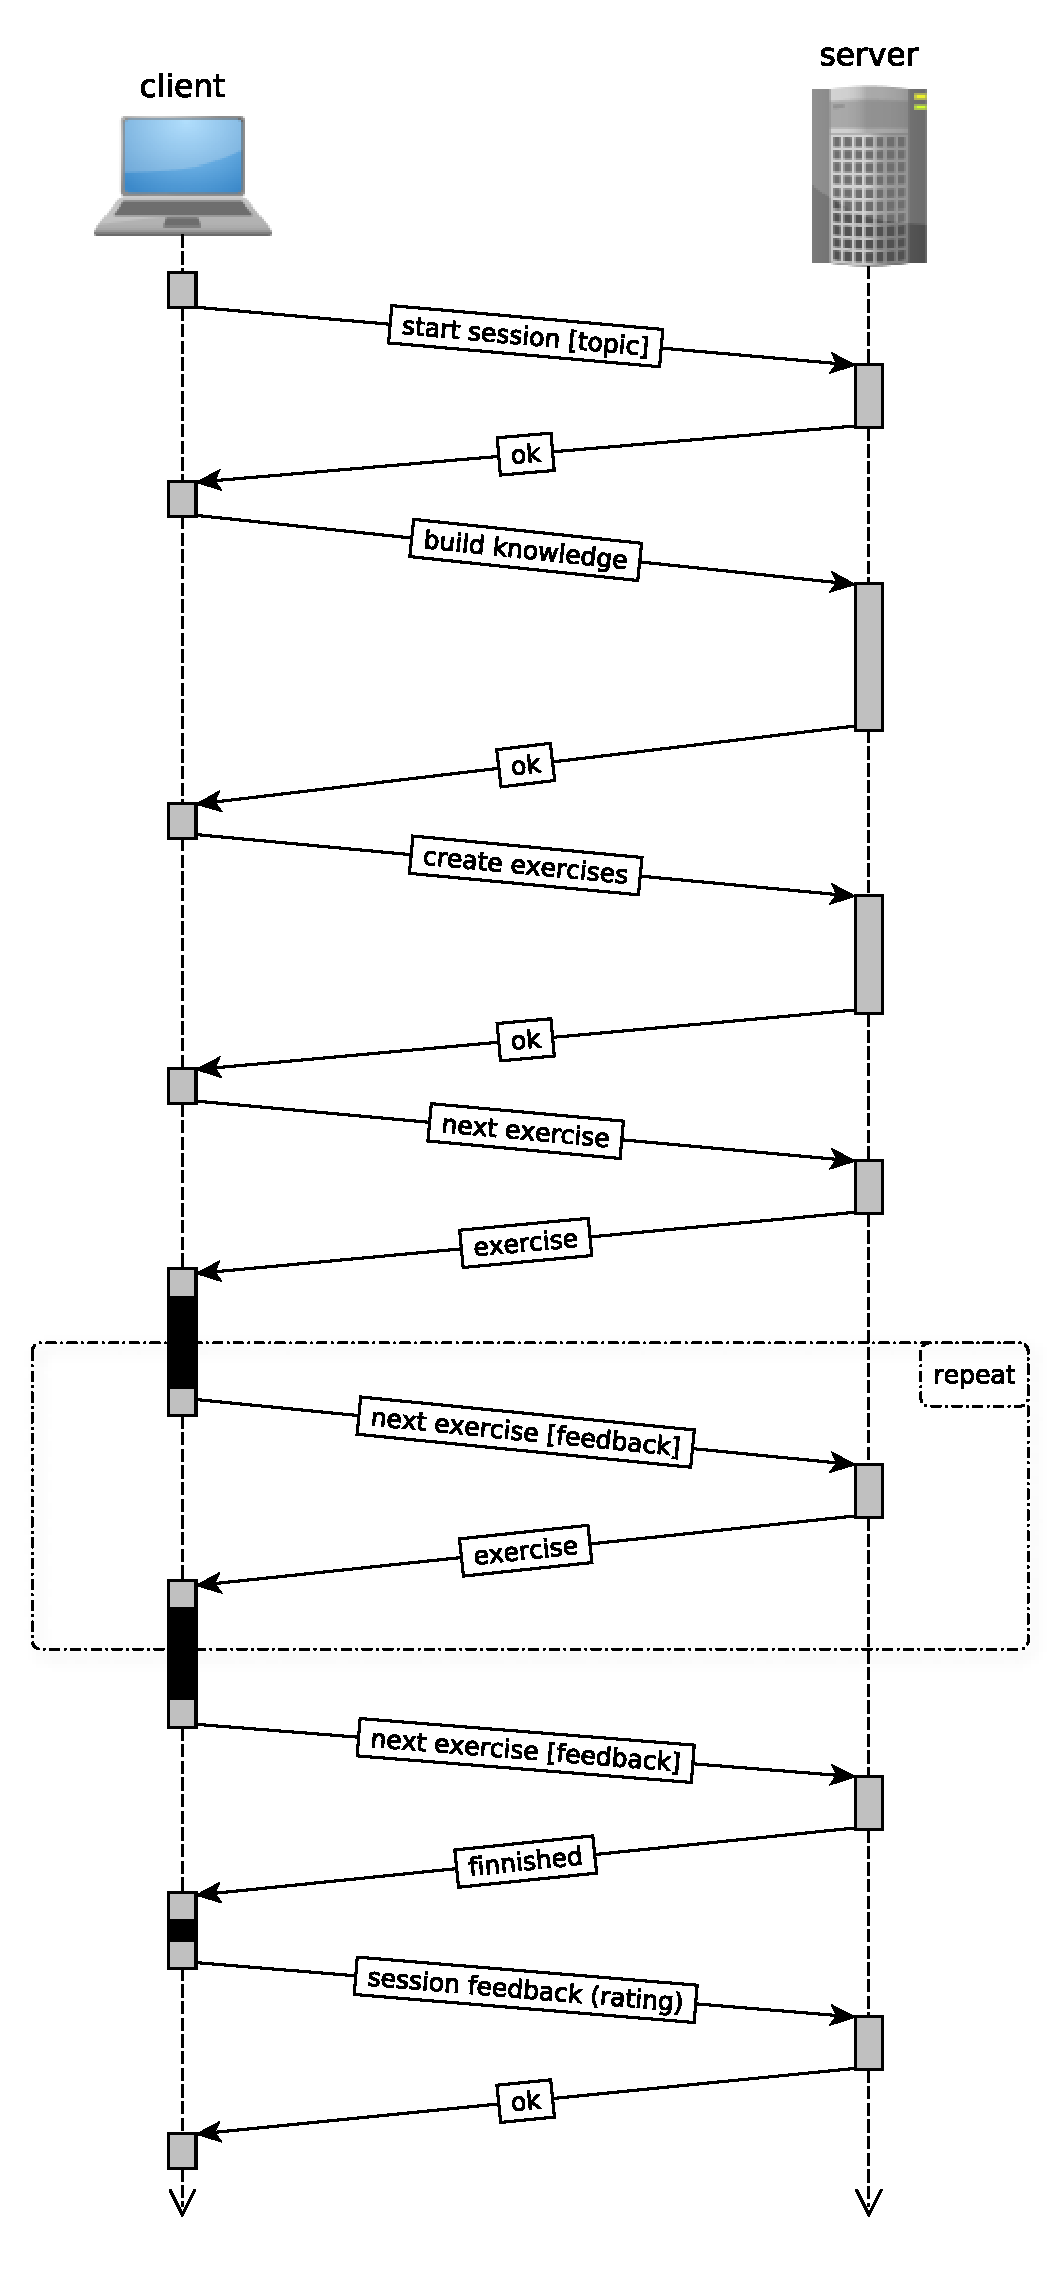
\includegraphics[width=0.66\textwidth]{images/client-server-communication.pdf}
  DONE
  \caption{Client-server communication}
  \label{fig:client-server-communication}
\end{figure}

\begin{figure}[h]
  \centering
  %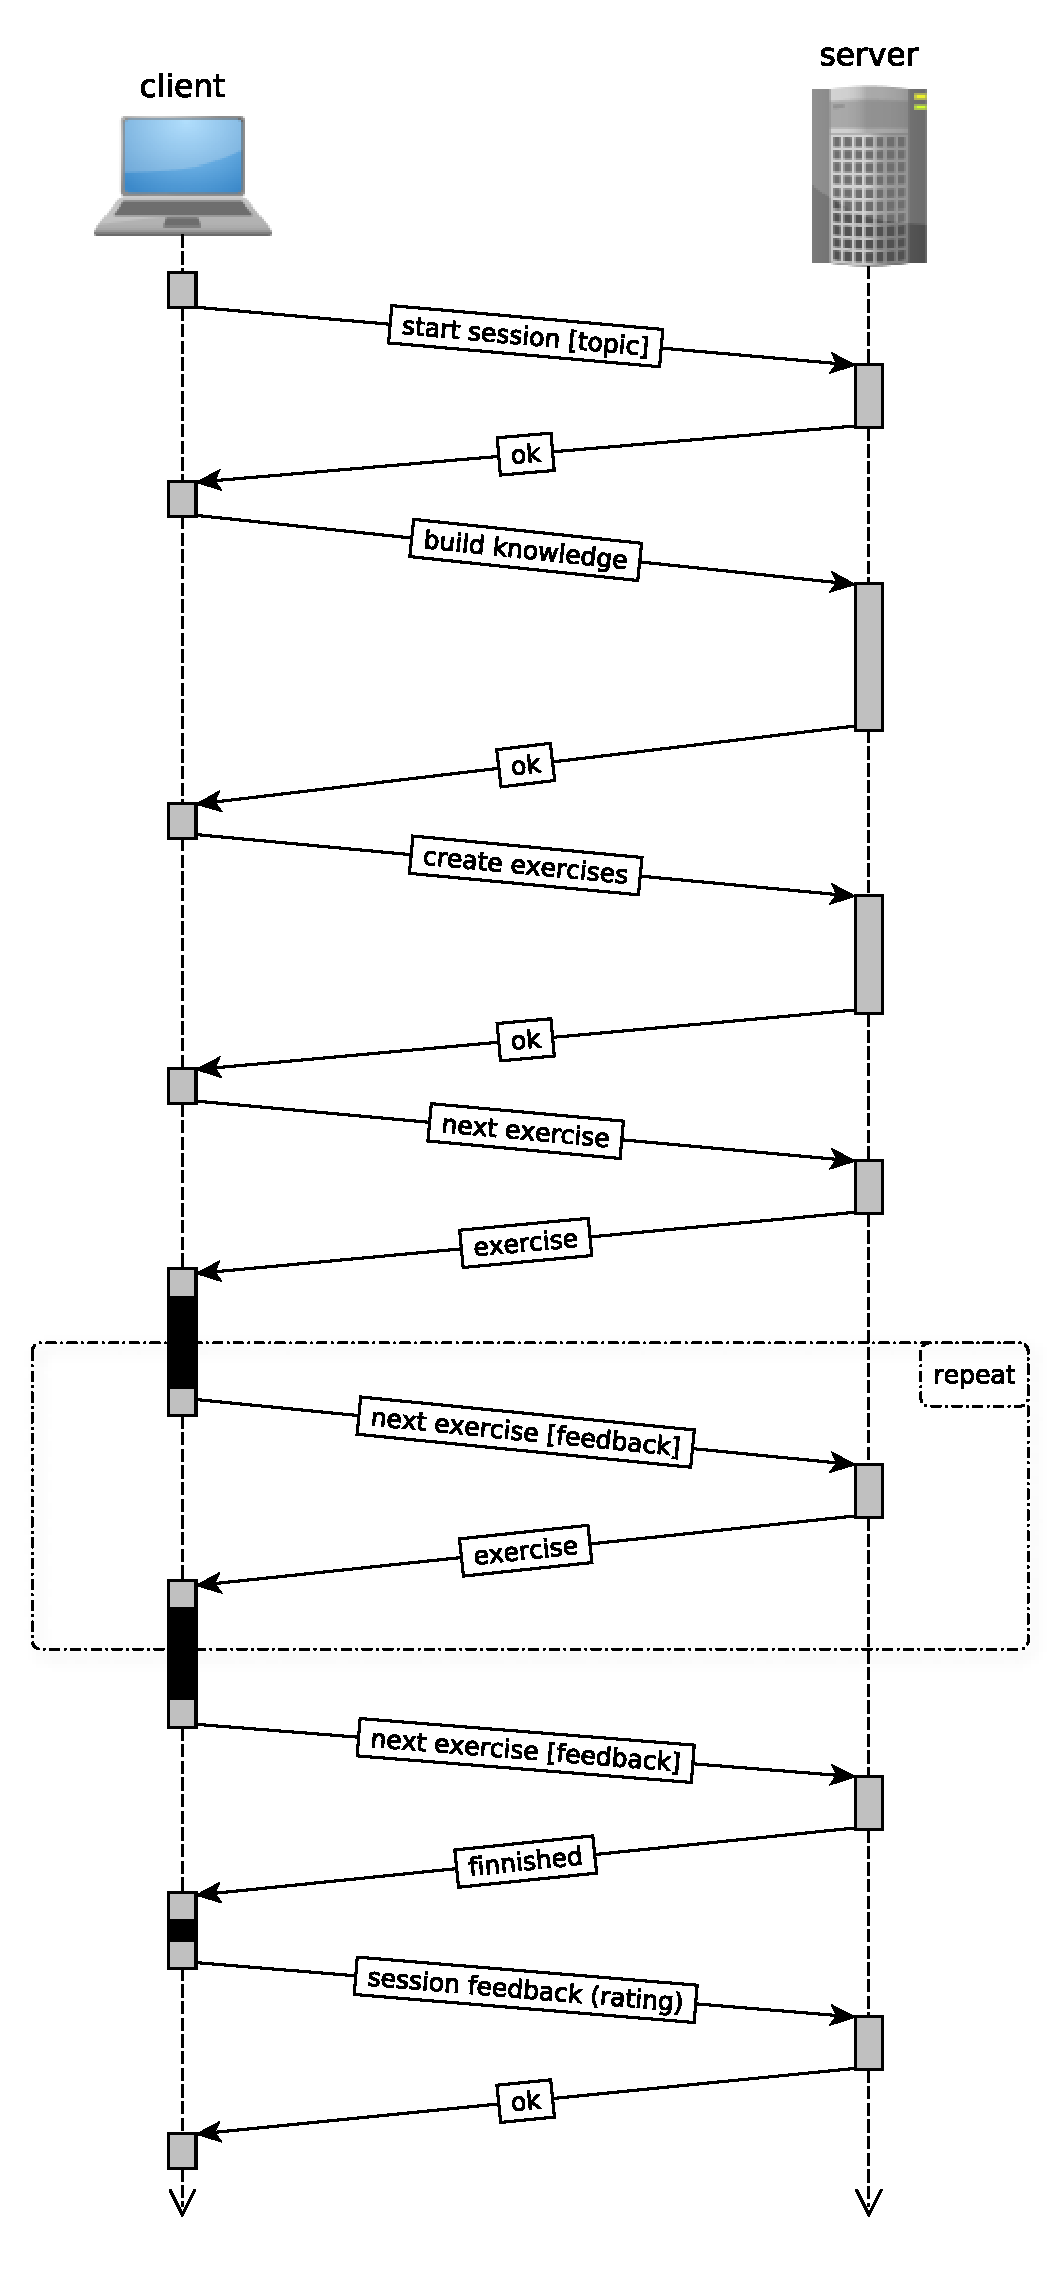
\includegraphics[width=0.66\textwidth]{images/client-server-communication.pdf}
  TODO ...
  \caption{Data flow diagram}
  \label{fig:data-flow-diagram}
\end{figure}

\begin{figure}[h]
  \centering
  %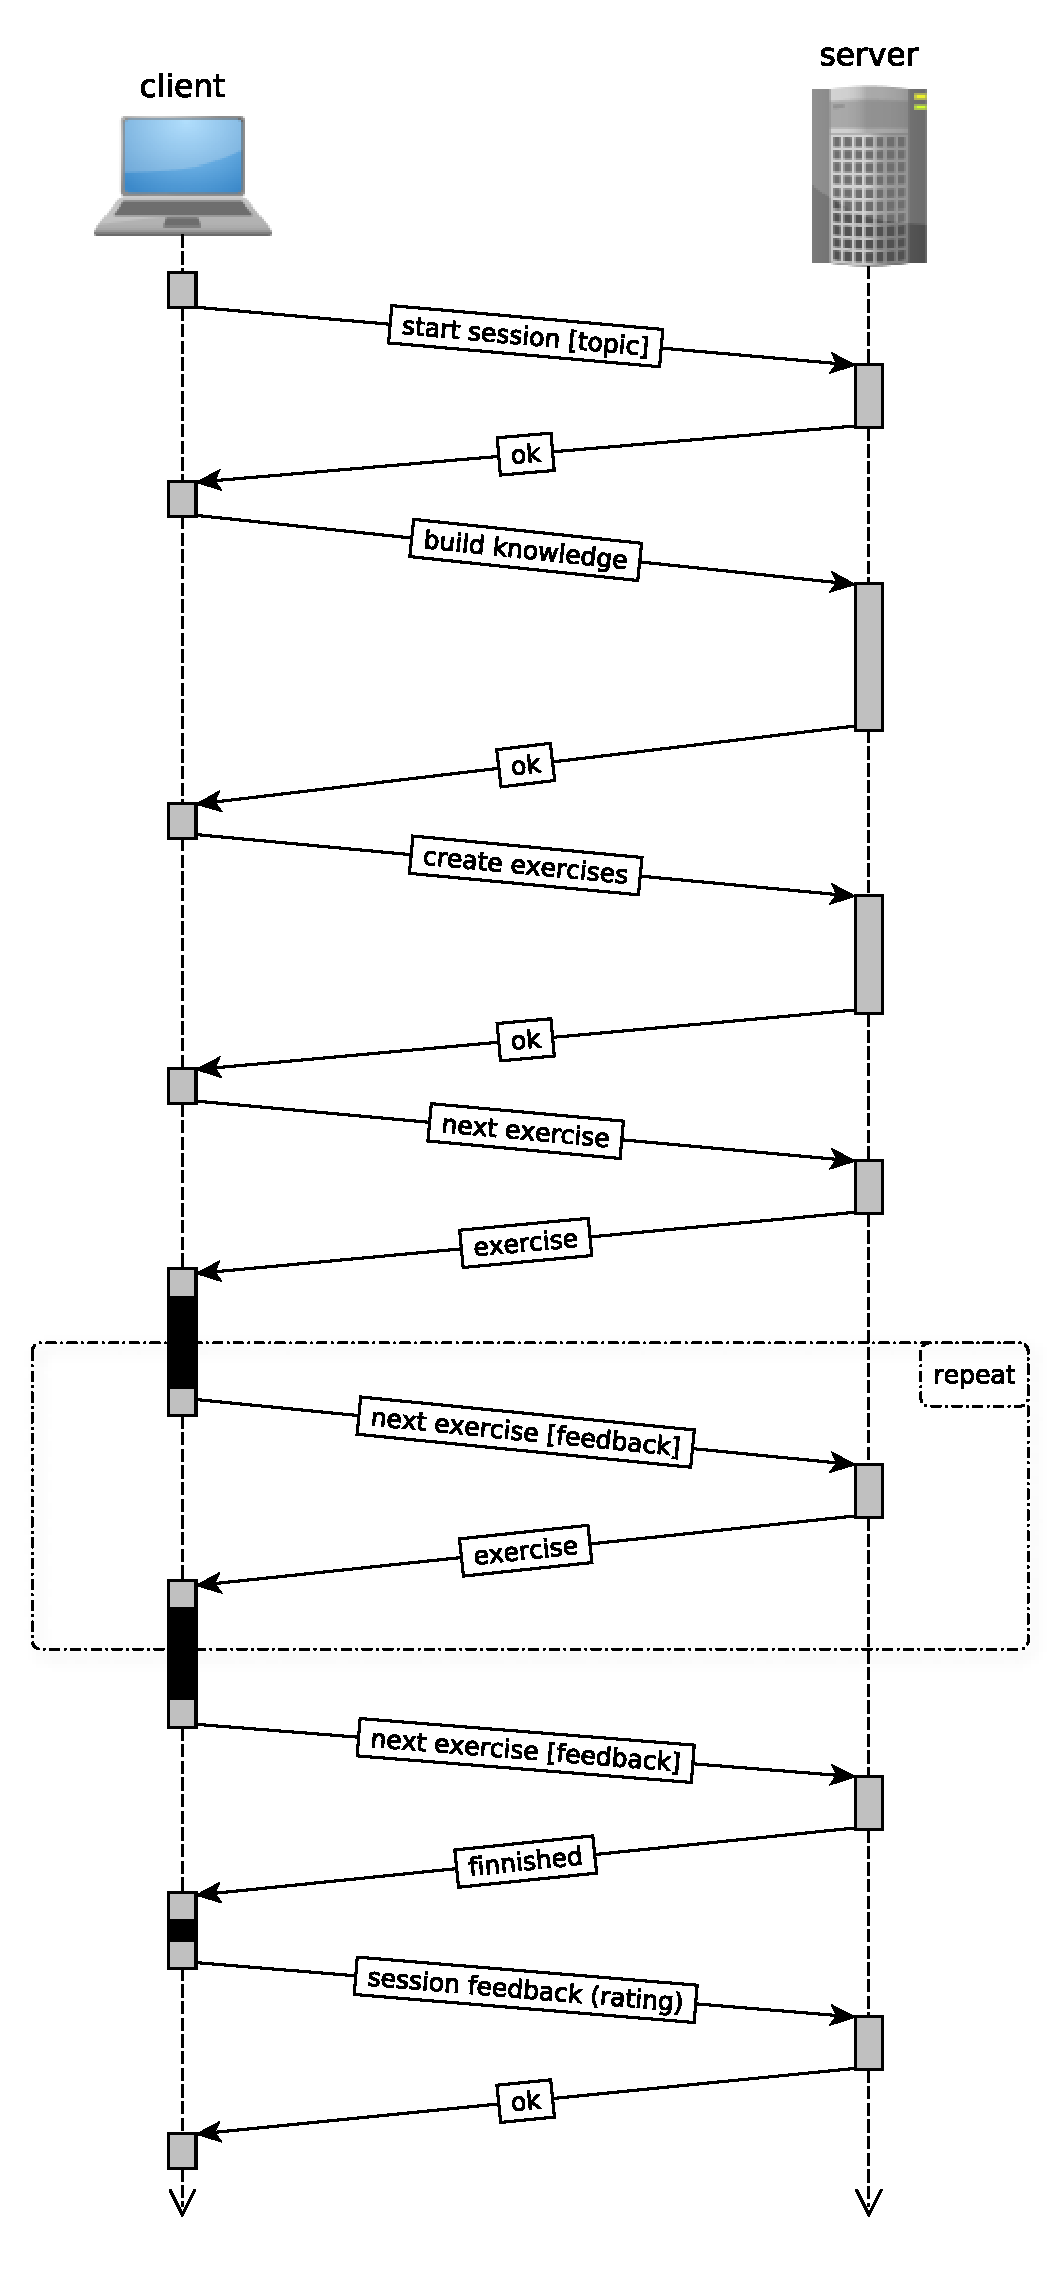
\includegraphics[width=0.66\textwidth]{images/client-server-communication.pdf}
  TODO ...
  \caption{Smartoo architecture}
  \label{fig:smartoo-architecture}
\end{figure}


\section{Knowledge Building}
\label{sec:smartoo-knowledge}

TODO...

\section{Exercises Creating}
\label{sec:smartoo-exercises}

TODO...

\section{Exercises Grading}
\label{sec:smartoo-exercises-grading}

TODO... obecne

\subsection{Component Interface}

TODO ...

\subsection{Prototype Behavior}

Grading is done via simple heuristics.

Difficulty of the exercise is estimated as the average similarity between all term pairs which can be mistaken (TODO: popsat prenos semanticke informace) (TODO: priklad paru u nejake otazky) (TODO: popis vypocu podobnosti 2 pojmu - bude vyse, takze jen odkazat).

(TODO: proc bylo zvoleno toto, vyhody, nevyhody.)

Relevance of the exercise is estimated as the cosine similarity meassure between the exercise and the article.
(TODO: popsat poradne, jak chapeme reprezentujem cviceni a clanek jako dokumenty, ze bereme jen pojmy...)

Cosine similarity between two documents (in our case one document is the article $A$ and another is the exercise $E$) is given by the following formula:
$$
similarity(A, E)
= \frac{A \cdot E}{|A| |E|}
= \frac{\sum_{i=1}^{n} A_i E_i}{\sqrt{\sum_{i=1}^{n} A_i^2}\sqrt{\sum_{i=1}^{n} E_i^2}}
$$
where $A_i$ ($E_i$) denotes numbers of occurences of the $i$-th term in article (exercise).
(TODO: odkaz na popis, interpretaci a zduvodneni cosine similarity, napr. z IRT)
(TODO: proc "cosine" -- jedna se cosinus uhlu mezi vektory 2 dokumentu)
(TODO: proc bylo zvoleno toto (napr. mezi 0 a 1, normalizace vzhledem k ruznym delkem, vyhody, nevyhody.)

\section{Adaptive Practice}
\label{sec:smartoo-practice}

TODO... obecne

\subsection{Component Interface}

TODO ...

\subsection{Prototype Behavior}

Implemented behavior of adaptive practicer is a .... (jak modeluje studenta... spis nijak, proste se snazim cilit na pozadovanou pravdepodobnost uspechu / simple heuristic...)

To select the most suitable exercise, three attributes of exercises are considered:

\begin{myItemize}
  \item relevance to the article,
  \item difficulty (compared to the so far success of the user),
  \item repetitiveness (to not ask about one term over and over again).
\end{myItemize}

Weights of these three attributes as well as the target success
are given by the behavior parameters.

\begin{table}[h]
\begin{center}
\begin{tabular}{| l | c | r | r |  r  |  r |  r |}
  \hline
  parameter & symbol & \multicolumn{5}{|c|}{used values} \\
  \hline \hline
  target success & $\tau$           & $0.75$ & $0.75$ & $0.75$ & $0.75$ & $0.75$\\ \hline
  relevance weight & $\alpha$      & $1.00$ & $1.25$ & $1.00$ & $1.00$ & $1.25$\\ \hline
  difficulty weight & $\beta$      & $1.00$ & $1.00$ & $1.25$ & $1.00$ & $1.00$\\ \hline
  repetitiveness weight & $\gamma$ & $0.25$ & $0.25$ & $0.25$ & $0.50$ & $0.50$\\ \hline
\end{tabular}
\end{center}
\caption{Parameters of prototype adaptive practice behavior}
\end{table}

Relevance of the exercise was computed by \textit{ExercisesGrade} (see (TODO: odkaz)).

Difficulty penalization is based on the difference between the target difficulty and the exercise difficulty.
Target difficulty is not exactly $(1 - \tau)$ as it is adjusted according to
so far success of the user -- if the correct ratio of the user is higher than the target success,
the target difficulty is set higher than $(1 - \tau)$ and vice versa.
(TODO: odkaz na experimenty na slepych mapach, kde se tohle ukazalo jako uzitecne)
(TODO: konkretni vzorec podle zdrojaku)

Repetitiveness penalization is based on the cosine similarity between the scored exercise and the exercises already used in the current session (TODO: odkaz na vysvetleni cosine similarity drive).

The total score is given as weighted sum of the three individual scores described above.
$$
\text{totalScore} = \alpha \cdot \text{relevanceScore} + \beta \cdot \text{difficultyPenalty} + \gamma \cdot \text{repetitivenessPenalty}
$$
An exercise with the highest score is chosen.


\section{Web Interface}
\label{sec:smartoo-web}

TODO...

\begin{figure}[h]
  \centering
  
\includegraphics[width=0.9\textwidth]{images/home-page.png}
  \caption{Smartoo home page}
  \label{fig:smartoo-home}
\end{figure}

\begin{figure}[h]
  \centering
  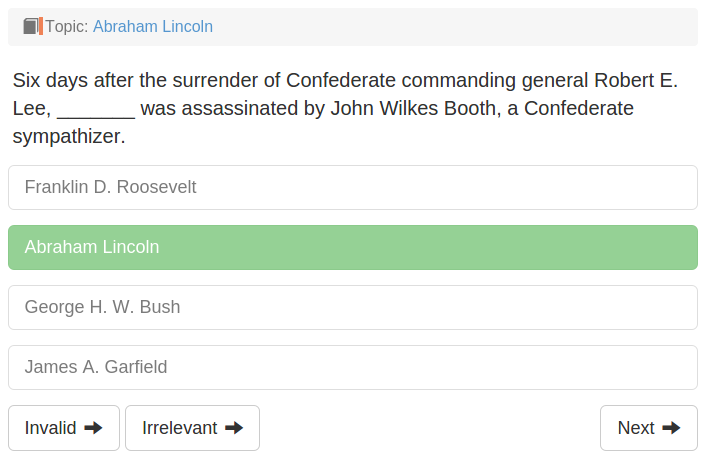
\includegraphics[width=0.9\textwidth]{images/answered-correctly.png}
  \caption{Correctly answered question}
  \label{fig:correctly-answered-question}
\end{figure}


% ===========================  CHAPTER ===========================
\chapter{Deployment and Evaluation}
\label{chap:evaluation}

TODO...

performace of each component

TODO: bylo by pekne, kdybych mohl ze ziskanych dat take zmerit RMSE tech 6 ruznych pracitce komponent (resp. te jejich casti, ktera modeluje studenta, tj. jak moc dobre ohdaduji, ze to uzivatel zvladne)

\chapter{Conclusions and Future Plans}
\label{chap:future}

TODO: strucne shrnuti a hlavne zavery na zaklade statistik a strucne budouci plany...


what to improve (... in diploma thesis)





% ===== APPENDIX AND BIBLIOGRAPHY =====
\appendix

% include citations not cited specifically
%\nocite{*}

% print complete bibliography
\printbibliography

\chapter{Data attachment}

TODO: data attachment structure description

\end{document}
